\begin{priprava}{3., 4}{}{Razdalja med točkama in razpolovišče daljice}{Pravokotni koordinatni sistem}{frontalna}{drsnice, projekcija, tabla}


    
    \section{Razdalja med točkama in razpolovišče daljice}

    
        \subsection*{Razdalja med točkama}

            \begin{wrapfigure}{r}{0.44\textwidth}
                \vskip-2em
                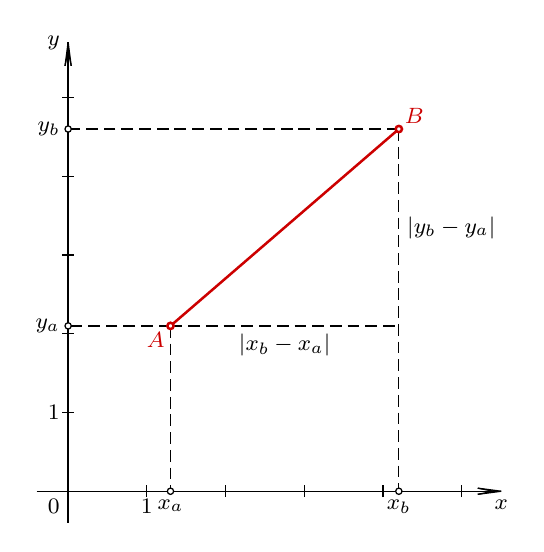
\begin{tikzpicture}
                    % \clip (0,0) rectangle (14.000000,10.000000);
                    {\footnotesize
                    
                    % Drawing 2D Cartesian system
                    \draw (2.000000,2.000000) node [anchor=north east] { $0$ };%
                    \draw [line width=0.016cm] (2.000000,1.925000) -- (2.000000,2.075000);%
                    \draw (3.000000,2.000000) node [anchor=north] { $1$ };%
                    \draw [line width=0.016cm] (3.000000,1.925000) -- (3.000000,2.075000);%
                    % \draw (4.000000,2.000000) node [anchor=north] { $2$ };%
                    \draw [line width=0.016cm] (4.000000,1.925000) -- (4.000000,2.075000);%
                    % \draw (5.000000,2.000000) node [anchor=north] { $3$ };%
                    \draw [line width=0.016cm] (5.000000,1.925000) -- (5.000000,2.075000);%
                    % \draw (6.000000,2.000000) node [anchor=north] { $4$ };%
                    \draw [line width=0.016cm] (6.000000,1.925000) -- (6.000000,2.075000);%
                    % \draw (7.000000,2.000000) node [anchor=north] { $5$ };%
                    \draw [line width=0.016cm] (7.000000,1.925000) -- (7.000000,2.075000);%
                    \draw (2.000000,3.000000) node [anchor=east] { $1$ };%
                    \draw [line width=0.016cm] (1.925000,3.000000) -- (2.075000,3.000000);%
                    % \draw (2.000000,4.000000) node [anchor=east] { $2$ };%
                    \draw [line width=0.016cm] (1.925000,4.000000) -- (2.075000,4.000000);%
                    % \draw (2.000000,5.000000) node [anchor=east] { $3$ };%
                    \draw [line width=0.016cm] (1.925000,5.000000) -- (2.075000,5.000000);%
                    % \draw (2.000000,6.000000) node [anchor=east] { $4$ };%
                    \draw [line width=0.016cm] (1.925000,6.000000) -- (2.075000,6.000000);%
                    % \draw (2.000000,7.000000) node [anchor=east] { $5$ };%
                    \draw [line width=0.016cm] (1.925000,7.000000) -- (2.075000,7.000000);%
                    \draw (7.500000,2.000000) node [anchor=north] { $x$ };%
                    \draw (2.000000,7.700000) node [anchor=east] { $y$ };%
                    \draw [line width=0.016cm] (1.600000,2.000000) -- (3.260000,2.000000);%
                    \draw [line width=0.016cm] (3.340000,2.000000) -- (6.160000,2.000000);%
                    \draw [line width=0.016cm] (6.240000,2.000000) -- (7.500000,2.000000);%
                    \draw [line width=0.016cm] (7.202567,2.039158) -- (7.500000,2.000000);%
                    \draw [line width=0.016cm] (7.202567,2.039158) -- (7.400000,2.000000);%
                    \draw [line width=0.016cm] (7.202567,1.960842) -- (7.500000,2.000000);%
                    \draw [line width=0.016cm] (7.202567,1.960842) -- (7.400000,2.000000);%
                    \draw [line width=0.016cm] (2.000000,1.600000) -- (2.000000,4.060000);%
                    \draw [line width=0.016cm] (2.000000,4.140000) -- (2.000000,6.560000);%
                    \draw [line width=0.016cm] (2.000000,6.640000) -- (2.000000,7.700000);%
                    \draw [line width=0.016cm] (1.960842,7.402567) -- (2.000000,7.700000);%
                    \draw [line width=0.016cm] (1.960842,7.402567) -- (2.000000,7.600000);%
                    \draw [line width=0.016cm] (2.039158,7.402567) -- (2.000000,7.700000);%
                    \draw [line width=0.016cm] (2.039158,7.402567) -- (2.000000,7.600000);%
                    
                    % Drawing segment A x_a
                    \draw [line width=0.016cm] (3.300000,4.060000) -- (3.300000,3.950000);%
                    \draw [line width=0.016cm] (3.300000,3.875000) -- (3.300000,3.725000);%
                    \draw [line width=0.016cm] (3.300000,3.650000) -- (3.300000,3.500000);%
                    \draw [line width=0.016cm] (3.300000,3.425000) -- (3.300000,3.275000);%
                    \draw [line width=0.016cm] (3.300000,3.200000) -- (3.300000,3.050000);%
                    \draw [line width=0.016cm] (3.300000,2.975000) -- (3.300000,2.825000);%
                    \draw [line width=0.016cm] (3.300000,2.750000) -- (3.300000,2.600000);%
                    \draw [line width=0.016cm] (3.300000,2.525000) -- (3.300000,2.375000);%
                    \draw [line width=0.016cm] (3.300000,2.300000) -- (3.300000,2.150000);%
                    \draw [line width=0.016cm] (3.300000,2.075000) -- (3.300000,2.040000);%
                    
                    % Drawing segment A y_a
                    \draw [line width=0.016cm] (3.260000,4.100000) -- (3.150000,4.100000);%
                    \draw [line width=0.016cm] (3.075000,4.100000) -- (2.925000,4.100000);%
                    \draw [line width=0.016cm] (2.850000,4.100000) -- (2.700000,4.100000);%
                    \draw [line width=0.016cm] (2.625000,4.100000) -- (2.475000,4.100000);%
                    \draw [line width=0.016cm] (2.400000,4.100000) -- (2.250000,4.100000);%
                    \draw [line width=0.016cm] (2.175000,4.100000) -- (2.040000,4.100000);%
                    
                    % Drawing segment B x_b
                    \draw [line width=0.016cm] (6.200000,6.560000) -- (6.200000,6.450000);%
                    \draw [line width=0.016cm] (6.200000,6.375000) -- (6.200000,6.225000);%
                    \draw [line width=0.016cm] (6.200000,6.150000) -- (6.200000,6.000000);%
                    \draw [line width=0.016cm] (6.200000,5.925000) -- (6.200000,5.775000);%
                    \draw [line width=0.016cm] (6.200000,5.700000) -- (6.200000,5.550000);%
                    \draw [line width=0.016cm] (6.200000,5.475000) -- (6.200000,5.325000);%
                    \draw [line width=0.016cm] (6.200000,5.250000) -- (6.200000,5.100000);%
                    \draw [line width=0.016cm] (6.200000,5.025000) -- (6.200000,4.875000);%
                    \draw [line width=0.016cm] (6.200000,4.800000) -- (6.200000,4.650000);%
                    \draw [line width=0.016cm] (6.200000,4.575000) -- (6.200000,4.425000);%
                    \draw [line width=0.016cm] (6.200000,4.350000) -- (6.200000,4.200000);%
                    \draw [line width=0.016cm] (6.200000,4.125000) -- (6.200000,3.975000);%
                    \draw [line width=0.016cm] (6.200000,3.900000) -- (6.200000,3.750000);%
                    \draw [line width=0.016cm] (6.200000,3.675000) -- (6.200000,3.525000);%
                    \draw [line width=0.016cm] (6.200000,3.450000) -- (6.200000,3.300000);%
                    \draw [line width=0.016cm] (6.200000,3.225000) -- (6.200000,3.075000);%
                    \draw [line width=0.016cm] (6.200000,3.000000) -- (6.200000,2.850000);%
                    \draw [line width=0.016cm] (6.200000,2.775000) -- (6.200000,2.625000);%
                    \draw [line width=0.016cm] (6.200000,2.550000) -- (6.200000,2.400000);%
                    \draw [line width=0.016cm] (6.200000,2.325000) -- (6.200000,2.175000);%
                    \draw [line width=0.016cm] (6.200000,2.100000) -- (6.200000,2.040000);%
                    
                    % Drawing segment B y_b
                    \draw [line width=0.016cm] (6.160000,6.600000) -- (6.050000,6.600000);%
                    \draw [line width=0.016cm] (5.975000,6.600000) -- (5.825000,6.600000);%
                    \draw [line width=0.016cm] (5.750000,6.600000) -- (5.600000,6.600000);%
                    \draw [line width=0.016cm] (5.525000,6.600000) -- (5.375000,6.600000);%
                    \draw [line width=0.016cm] (5.300000,6.600000) -- (5.150000,6.600000);%
                    \draw [line width=0.016cm] (5.075000,6.600000) -- (4.925000,6.600000);%
                    \draw [line width=0.016cm] (4.850000,6.600000) -- (4.700000,6.600000);%
                    \draw [line width=0.016cm] (4.625000,6.600000) -- (4.475000,6.600000);%
                    \draw [line width=0.016cm] (4.400000,6.600000) -- (4.250000,6.600000);%
                    \draw [line width=0.016cm] (4.175000,6.600000) -- (4.025000,6.600000);%
                    \draw [line width=0.016cm] (3.950000,6.600000) -- (3.800000,6.600000);%
                    \draw [line width=0.016cm] (3.725000,6.600000) -- (3.575000,6.600000);%
                    \draw [line width=0.016cm] (3.500000,6.600000) -- (3.350000,6.600000);%
                    \draw [line width=0.016cm] (3.275000,6.600000) -- (3.125000,6.600000);%
                    \draw [line width=0.016cm] (3.050000,6.600000) -- (2.900000,6.600000);%
                    \draw [line width=0.016cm] (2.825000,6.600000) -- (2.675000,6.600000);%
                    \draw [line width=0.016cm] (2.600000,6.600000) -- (2.450000,6.600000);%
                    \draw [line width=0.016cm] (2.375000,6.600000) -- (2.225000,6.600000);%
                    \draw [line width=0.016cm] (2.150000,6.600000) -- (2.040000,6.600000);%
                    
                    % Drawing segment A xy
                    \draw [line width=0.016cm] (3.340000,4.100000) -- (3.450000,4.100000);%
                    \draw [line width=0.016cm] (3.525000,4.100000) -- (3.675000,4.100000);%
                    \draw [line width=0.016cm] (3.750000,4.100000) -- (3.900000,4.100000);%
                    \draw [line width=0.016cm] (3.975000,4.100000) -- (4.125000,4.100000);%
                    \draw [line width=0.016cm] (4.200000,4.100000) -- (4.350000,4.100000);%
                    \draw [line width=0.016cm] (4.425000,4.100000) -- (4.575000,4.100000);%
                    \draw [line width=0.016cm] (4.650000,4.100000) -- (4.800000,4.100000);%
                    \draw [line width=0.016cm] (4.875000,4.100000) -- (5.025000,4.100000);%
                    \draw [line width=0.016cm] (5.100000,4.100000) -- (5.250000,4.100000);%
                    \draw [line width=0.016cm] (5.325000,4.100000) -- (5.475000,4.100000);%
                    \draw [line width=0.016cm] (5.550000,4.100000) -- (5.700000,4.100000);%
                    \draw [line width=0.016cm] (5.775000,4.100000) -- (5.925000,4.100000);%
                    \draw [line width=0.016cm] (6.000000,4.100000) -- (6.150000,4.100000);%
                    
                    % Marking point x_a by circle
                    \draw [line width=0.016cm] (3.300000,2.000000) circle (0.040000);%
                    \draw (3.300000,2.000000) node [anchor=north] { $x_a$ };%
                    
                    % Marking point x_b by circle
                    \draw [line width=0.016cm] (6.200000,2.000000) circle (0.040000);%
                    \draw (6.200000,2.000000) node [anchor=north] { $x_b$ };%
                    
                    % Marking point y_a by circle
                    \draw [line width=0.016cm] (2.000000,4.100000) circle (0.040000);%
                    \draw (2.000000,4.100000) node [anchor=east] { $y_a$ };%
                    
                    % Marking point y_b by circle
                    \draw [line width=0.016cm] (2.000000,6.600000) circle (0.040000);%
                    \draw (2.000000,6.600000) node [anchor=east] { $y_b$ };%
                    
                    % Marking point {|x_b-x_a|}
                    \draw (4.750000,4.100000) node [anchor=north] { ${|x_b-x_a|}$ };%
                    
                    % Marking point {|y_b-y_a|}
                    \draw (6.200000,5.350000) node [anchor=west] { ${|y_b-y_a|}$ };%
                    
                    % Changing color 204 0 0
                    \definecolor{r204g0b0}{rgb}{0.800000,0.000000,0.000000}%
                    \color{r204g0b0}% 
                    
                    % Drawing segment A B
                    \draw [line width=0.032cm] (3.330296,4.126118) -- (6.169704,6.573882);%
                    
                    % Marking point A by circle
                    \draw [line width=0.032cm] (3.300000,4.100000) circle (0.040000);%
                    \draw (3.330000,4.130000) node [anchor=north east] { $A$ };%
                    
                    % Marking point B by circle
                    \draw [line width=0.032cm] (6.200000,6.600000) circle (0.040000);%
                    \draw (6.170000,6.570000) node [anchor=south west] { $B$ };%
                    \color{black}
                    }
                    \end{tikzpicture}

                    \begin{tikzpicture}
                        % \clip (0,0) rectangle (14.000000,10.000000);
                        {\footnotesize
                        
                        % Drawing 2D Cartesian system
                        \draw (2.000000,2.000000) node [anchor=north east] { $0$ };%
                        \draw [line width=0.016cm] (2.000000,1.925000) -- (2.000000,2.075000);%
                        \draw (3.000000,2.000000) node [anchor=north] { $1$ };%
                        \draw [line width=0.016cm] (3.000000,1.925000) -- (3.000000,2.075000);%
                        % \draw (4.000000,2.000000) node [anchor=north] { $2$ };%
                        \draw [line width=0.016cm] (4.000000,1.925000) -- (4.000000,2.075000);%
                        % \draw (5.000000,2.000000) node [anchor=north] { $3$ };%
                        \draw [line width=0.016cm] (5.000000,1.925000) -- (5.000000,2.075000);%
                        % \draw (6.000000,2.000000) node [anchor=north] { $4$ };%
                        \draw [line width=0.016cm] (6.000000,1.925000) -- (6.000000,2.075000);%
                        % \draw (7.000000,2.000000) node [anchor=north] { $5$ };%
                        \draw [line width=0.016cm] (7.000000,1.925000) -- (7.000000,2.075000);%
                        \draw (2.000000,3.000000) node [anchor=east] { $1$ };%
                        \draw [line width=0.016cm] (1.925000,3.000000) -- (2.075000,3.000000);%
                        % \draw (2.000000,4.000000) node [anchor=east] { $2$ };%
                        \draw [line width=0.016cm] (1.925000,4.000000) -- (2.075000,4.000000);%
                        % \draw (2.000000,5.000000) node [anchor=east] { $3$ };%
                        \draw [line width=0.016cm] (1.925000,5.000000) -- (2.075000,5.000000);%
                        % \draw (2.000000,6.000000) node [anchor=east] { $4$ };%
                        \draw [line width=0.016cm] (1.925000,6.000000) -- (2.075000,6.000000);%
                        % \draw (2.000000,7.000000) node [anchor=east] { $5$ };%
                        \draw [line width=0.016cm] (1.925000,7.000000) -- (2.075000,7.000000);%
                        \draw (7.500000,2.000000) node [anchor=north] { $x$ };%
                        \draw (2.000000,7.400000) node [anchor=east] { $y$ };%
                        \draw [line width=0.016cm] (1.300000,2.000000) -- (3.260000,2.000000);%
                        \draw [line width=0.016cm] (3.340000,2.000000) -- (4.710000,2.000000);%
                        \draw [line width=0.016cm] (4.790000,2.000000) -- (6.160000,2.000000);%
                        \draw [line width=0.016cm] (6.240000,2.000000) -- (7.500000,2.000000);%
                        \draw [line width=0.016cm] (7.202567,2.039158) -- (7.500000,2.000000);%
                        \draw [line width=0.016cm] (7.202567,2.039158) -- (7.400000,2.000000);%
                        \draw [line width=0.016cm] (7.202567,1.960842) -- (7.500000,2.000000);%
                        \draw [line width=0.016cm] (7.202567,1.960842) -- (7.400000,2.000000);%
                        \draw [line width=0.016cm] (2.000000,1.300000) -- (2.000000,4.060000);%
                        \draw [line width=0.016cm] (2.000000,4.140000) -- (2.000000,5.310000);%
                        \draw [line width=0.016cm] (2.000000,5.390000) -- (2.000000,6.560000);%
                        \draw [line width=0.016cm] (2.000000,6.640000) -- (2.000000,7.400000);%
                        \draw [line width=0.016cm] (1.960842,7.102567) -- (2.000000,7.400000);%
                        \draw [line width=0.016cm] (1.960842,7.102567) -- (2.000000,7.300000);%
                        \draw [line width=0.016cm] (2.039158,7.102567) -- (2.000000,7.400000);%
                        \draw [line width=0.016cm] (2.039158,7.102567) -- (2.000000,7.300000);%
                        
                        % Drawing segment A x_a
                        \draw [line width=0.016cm] (3.300000,4.060000) -- (3.300000,3.950000);%
                        \draw [line width=0.016cm] (3.300000,3.875000) -- (3.300000,3.725000);%
                        \draw [line width=0.016cm] (3.300000,3.650000) -- (3.300000,3.500000);%
                        \draw [line width=0.016cm] (3.300000,3.425000) -- (3.300000,3.275000);%
                        \draw [line width=0.016cm] (3.300000,3.200000) -- (3.300000,3.050000);%
                        \draw [line width=0.016cm] (3.300000,2.975000) -- (3.300000,2.825000);%
                        \draw [line width=0.016cm] (3.300000,2.750000) -- (3.300000,2.600000);%
                        \draw [line width=0.016cm] (3.300000,2.525000) -- (3.300000,2.375000);%
                        \draw [line width=0.016cm] (3.300000,2.300000) -- (3.300000,2.150000);%
                        \draw [line width=0.016cm] (3.300000,2.075000) -- (3.300000,2.040000);%
                        
                        % Drawing segment A y_a
                        \draw [line width=0.016cm] (3.260000,4.100000) -- (3.150000,4.100000);%
                        \draw [line width=0.016cm] (3.075000,4.100000) -- (2.925000,4.100000);%
                        \draw [line width=0.016cm] (2.850000,4.100000) -- (2.700000,4.100000);%
                        \draw [line width=0.016cm] (2.625000,4.100000) -- (2.475000,4.100000);%
                        \draw [line width=0.016cm] (2.400000,4.100000) -- (2.250000,4.100000);%
                        \draw [line width=0.016cm] (2.175000,4.100000) -- (2.040000,4.100000);%
                        
                        % Drawing segment B x_b
                        \draw [line width=0.016cm] (6.200000,6.560000) -- (6.200000,6.450000);%
                        \draw [line width=0.016cm] (6.200000,6.375000) -- (6.200000,6.225000);%
                        \draw [line width=0.016cm] (6.200000,6.150000) -- (6.200000,6.000000);%
                        \draw [line width=0.016cm] (6.200000,5.925000) -- (6.200000,5.775000);%
                        \draw [line width=0.016cm] (6.200000,5.700000) -- (6.200000,5.550000);%
                        \draw [line width=0.016cm] (6.200000,5.475000) -- (6.200000,5.325000);%
                        \draw [line width=0.016cm] (6.200000,5.250000) -- (6.200000,5.100000);%
                        \draw [line width=0.016cm] (6.200000,5.025000) -- (6.200000,4.875000);%
                        \draw [line width=0.016cm] (6.200000,4.800000) -- (6.200000,4.650000);%
                        \draw [line width=0.016cm] (6.200000,4.575000) -- (6.200000,4.425000);%
                        \draw [line width=0.016cm] (6.200000,4.350000) -- (6.200000,4.200000);%
                        \draw [line width=0.016cm] (6.200000,4.125000) -- (6.200000,3.975000);%
                        \draw [line width=0.016cm] (6.200000,3.900000) -- (6.200000,3.750000);%
                        \draw [line width=0.016cm] (6.200000,3.675000) -- (6.200000,3.525000);%
                        \draw [line width=0.016cm] (6.200000,3.450000) -- (6.200000,3.300000);%
                        \draw [line width=0.016cm] (6.200000,3.225000) -- (6.200000,3.075000);%
                        \draw [line width=0.016cm] (6.200000,3.000000) -- (6.200000,2.850000);%
                        \draw [line width=0.016cm] (6.200000,2.775000) -- (6.200000,2.625000);%
                        \draw [line width=0.016cm] (6.200000,2.550000) -- (6.200000,2.400000);%
                        \draw [line width=0.016cm] (6.200000,2.325000) -- (6.200000,2.175000);%
                        \draw [line width=0.016cm] (6.200000,2.100000) -- (6.200000,2.040000);%
                        
                        % Drawing segment B y_b
                        \draw [line width=0.016cm] (6.160000,6.600000) -- (6.050000,6.600000);%
                        \draw [line width=0.016cm] (5.975000,6.600000) -- (5.825000,6.600000);%
                        \draw [line width=0.016cm] (5.750000,6.600000) -- (5.600000,6.600000);%
                        \draw [line width=0.016cm] (5.525000,6.600000) -- (5.375000,6.600000);%
                        \draw [line width=0.016cm] (5.300000,6.600000) -- (5.150000,6.600000);%
                        \draw [line width=0.016cm] (5.075000,6.600000) -- (4.925000,6.600000);%
                        \draw [line width=0.016cm] (4.850000,6.600000) -- (4.700000,6.600000);%
                        \draw [line width=0.016cm] (4.625000,6.600000) -- (4.475000,6.600000);%
                        \draw [line width=0.016cm] (4.400000,6.600000) -- (4.250000,6.600000);%
                        \draw [line width=0.016cm] (4.175000,6.600000) -- (4.025000,6.600000);%
                        \draw [line width=0.016cm] (3.950000,6.600000) -- (3.800000,6.600000);%
                        \draw [line width=0.016cm] (3.725000,6.600000) -- (3.575000,6.600000);%
                        \draw [line width=0.016cm] (3.500000,6.600000) -- (3.350000,6.600000);%
                        \draw [line width=0.016cm] (3.275000,6.600000) -- (3.125000,6.600000);%
                        \draw [line width=0.016cm] (3.050000,6.600000) -- (2.900000,6.600000);%
                        \draw [line width=0.016cm] (2.825000,6.600000) -- (2.675000,6.600000);%
                        \draw [line width=0.016cm] (2.600000,6.600000) -- (2.450000,6.600000);%
                        \draw [line width=0.016cm] (2.375000,6.600000) -- (2.225000,6.600000);%
                        \draw [line width=0.016cm] (2.150000,6.600000) -- (2.040000,6.600000);%
                        
                        % Drawing segment S x_s
                        \draw [line width=0.016cm] (4.750000,5.310000) -- (4.750000,5.200000);%
                        \draw [line width=0.016cm] (4.750000,5.125000) -- (4.750000,4.975000);%
                        \draw [line width=0.016cm] (4.750000,4.900000) -- (4.750000,4.750000);%
                        \draw [line width=0.016cm] (4.750000,4.675000) -- (4.750000,4.525000);%
                        \draw [line width=0.016cm] (4.750000,4.450000) -- (4.750000,4.300000);%
                        \draw [line width=0.016cm] (4.750000,4.225000) -- (4.750000,4.075000);%
                        \draw [line width=0.016cm] (4.750000,4.000000) -- (4.750000,3.850000);%
                        \draw [line width=0.016cm] (4.750000,3.775000) -- (4.750000,3.625000);%
                        \draw [line width=0.016cm] (4.750000,3.550000) -- (4.750000,3.400000);%
                        \draw [line width=0.016cm] (4.750000,3.325000) -- (4.750000,3.175000);%
                        \draw [line width=0.016cm] (4.750000,3.100000) -- (4.750000,2.950000);%
                        \draw [line width=0.016cm] (4.750000,2.875000) -- (4.750000,2.725000);%
                        \draw [line width=0.016cm] (4.750000,2.650000) -- (4.750000,2.500000);%
                        \draw [line width=0.016cm] (4.750000,2.425000) -- (4.750000,2.275000);%
                        \draw [line width=0.016cm] (4.750000,2.200000) -- (4.750000,2.050000);%
                        
                        % Drawing segment S y_s
                        \draw [line width=0.016cm] (4.710000,5.350000) -- (4.600000,5.350000);%
                        \draw [line width=0.016cm] (4.525000,5.350000) -- (4.375000,5.350000);%
                        \draw [line width=0.016cm] (4.300000,5.350000) -- (4.150000,5.350000);%
                        \draw [line width=0.016cm] (4.075000,5.350000) -- (3.925000,5.350000);%
                        \draw [line width=0.016cm] (3.850000,5.350000) -- (3.700000,5.350000);%
                        \draw [line width=0.016cm] (3.625000,5.350000) -- (3.475000,5.350000);%
                        \draw [line width=0.016cm] (3.400000,5.350000) -- (3.250000,5.350000);%
                        \draw [line width=0.016cm] (3.175000,5.350000) -- (3.025000,5.350000);%
                        \draw [line width=0.016cm] (2.950000,5.350000) -- (2.800000,5.350000);%
                        \draw [line width=0.016cm] (2.725000,5.350000) -- (2.575000,5.350000);%
                        \draw [line width=0.016cm] (2.500000,5.350000) -- (2.350000,5.350000);%
                        \draw [line width=0.016cm] (2.275000,5.350000) -- (2.125000,5.350000);%
                        \draw [line width=0.016cm] (2.050000,5.350000) -- (2.040000,5.350000);%
                        
                        % Marking point x_a by circle
                        \draw [line width=0.016cm] (3.300000,2.000000) circle (0.040000);%
                        \draw (3.300000,2.000000) node [anchor=north] { $x_a$ };%
                        
                        % Marking point x_b by circle
                        \draw [line width=0.016cm] (6.200000,2.000000) circle (0.040000);%
                        \draw (6.200000,2.000000) node [anchor=north] { $x_b$ };%
                        
                        % Marking point y_a by circle
                        \draw [line width=0.016cm] (2.000000,4.100000) circle (0.040000);%
                        \draw (2.000000,4.100000) node [anchor=east] { $y_a$ };%
                        
                        % Marking point y_b by circle
                        \draw [line width=0.016cm] (2.000000,6.600000) circle (0.040000);%
                        \draw (2.000000,6.600000) node [anchor=east] { $y_b$ };%
                        
                        % Drawing segment A B
                        \draw [line width=0.032cm] (3.330296,4.126118) -- (4.719704,5.323882);%
                        \draw [line width=0.032cm] (4.780296,5.376118) -- (6.169704,6.573882);%
                        
                        % Marking point A by circle
                        \draw [line width=0.032cm] (3.300000,4.100000) circle (0.040000);%
                        \draw (3.330000,4.130000) node [anchor=north east] { $A$ };%
                        
                        % Marking point B by circle
                        \draw [line width=0.032cm] (6.200000,6.600000) circle (0.040000);%
                        \draw (6.170000,6.570000) node [anchor=south west] { $B$ };%
                        
                        % Changing color 204 0 0
                        \definecolor{r204g0b0}{rgb}{0.800000,0.000000,0.000000}%
                        \color{r204g0b0}% 
                        
                        % Marking point S by circle
                        \draw [line width=0.032cm] (4.750000,5.350000) circle (0.040000);%
                        \draw (4.780000,5.320000) node [anchor=south east] { $S$ };%
                        
                        % Marking point y_s by circle
                        \draw [line width=0.032cm] (2.000000,5.350000) circle (0.040000);%
                        \draw (2.000000,5.350000) node [anchor=east] { $\frac{y_a+y_b}{2}$ };%
                        
                        % Marking point x_s by circle
                        \draw [line width=0.032cm] (4.750000,2.000000) circle (0.040000);%
                        \draw (4.750000,2.000000) node [anchor=north] { $\frac{x_a+x_b}{2}$ };%
                        
                        \color{black}
                        }
                    \end{tikzpicture}
                        
            \end{wrapfigure}
        
            Razdalja $d(A,B)$ med dvema točkama $A(x_a,y_a)$ in $B(x_b,y_b)$ v ravnini je
            $$ d(A,B)=\sqrt{(x_b-x_a)^2+(y_b-y_a)^2}. $$
        

        \subsubsection*{Lastnosti razdalje}
            \begin{itemize}
                \item $d(A,B)\geq 0$
                \item $d(A,B)=0\Leftrightarrow A=B$
                \item $d(A,B)=d(B,A)$
                \item $d(A,C)\leq d(A,B)+d(B,C)$
            \end{itemize}

            ~\\~\\~
    
    
        \subsection*{Razpolovišče daljice}
        
                Razpolovišče $S$ daljice $AB$ s krajiščema $A(x_a,y_a)$ in $B(x_b,y_b)$ v ravnini je
                $$ S\left(\dfrac{x_a+x_b}{2},\dfrac{y_a+y_b}{2}\right). $$
            

            % \begin{figure}[H]
            %     \begin{tikzpicture}
            %         % \clip (0,0) rectangle (14.000000,10.000000);
            %         {\footnotesize
                    
            %         % Drawing 2D Cartesian system
            %         \draw (2.000000,2.000000) node [anchor=north east] { $0$ };%
            %         \draw [line width=0.016cm] (2.000000,1.925000) -- (2.000000,2.075000);%
            %         \draw (3.000000,2.000000) node [anchor=north] { $1$ };%
            %         \draw [line width=0.016cm] (3.000000,1.925000) -- (3.000000,2.075000);%
            %         % \draw (4.000000,2.000000) node [anchor=north] { $2$ };%
            %         \draw [line width=0.016cm] (4.000000,1.925000) -- (4.000000,2.075000);%
            %         % \draw (5.000000,2.000000) node [anchor=north] { $3$ };%
            %         \draw [line width=0.016cm] (5.000000,1.925000) -- (5.000000,2.075000);%
            %         % \draw (6.000000,2.000000) node [anchor=north] { $4$ };%
            %         \draw [line width=0.016cm] (6.000000,1.925000) -- (6.000000,2.075000);%
            %         % \draw (7.000000,2.000000) node [anchor=north] { $5$ };%
            %         \draw [line width=0.016cm] (7.000000,1.925000) -- (7.000000,2.075000);%
            %         \draw (2.000000,3.000000) node [anchor=east] { $1$ };%
            %         \draw [line width=0.016cm] (1.925000,3.000000) -- (2.075000,3.000000);%
            %         % \draw (2.000000,4.000000) node [anchor=east] { $2$ };%
            %         \draw [line width=0.016cm] (1.925000,4.000000) -- (2.075000,4.000000);%
            %         % \draw (2.000000,5.000000) node [anchor=east] { $3$ };%
            %         \draw [line width=0.016cm] (1.925000,5.000000) -- (2.075000,5.000000);%
            %         % \draw (2.000000,6.000000) node [anchor=east] { $4$ };%
            %         \draw [line width=0.016cm] (1.925000,6.000000) -- (2.075000,6.000000);%
            %         % \draw (2.000000,7.000000) node [anchor=east] { $5$ };%
            %         \draw [line width=0.016cm] (1.925000,7.000000) -- (2.075000,7.000000);%
            %         \draw (7.500000,2.000000) node [anchor=north] { $x$ };%
            %         \draw (2.000000,7.400000) node [anchor=east] { $y$ };%
            %         \draw [line width=0.016cm] (1.300000,2.000000) -- (3.260000,2.000000);%
            %         \draw [line width=0.016cm] (3.340000,2.000000) -- (4.710000,2.000000);%
            %         \draw [line width=0.016cm] (4.790000,2.000000) -- (6.160000,2.000000);%
            %         \draw [line width=0.016cm] (6.240000,2.000000) -- (7.500000,2.000000);%
            %         \draw [line width=0.016cm] (7.202567,2.039158) -- (7.500000,2.000000);%
            %         \draw [line width=0.016cm] (7.202567,2.039158) -- (7.400000,2.000000);%
            %         \draw [line width=0.016cm] (7.202567,1.960842) -- (7.500000,2.000000);%
            %         \draw [line width=0.016cm] (7.202567,1.960842) -- (7.400000,2.000000);%
            %         \draw [line width=0.016cm] (2.000000,1.300000) -- (2.000000,4.060000);%
            %         \draw [line width=0.016cm] (2.000000,4.140000) -- (2.000000,5.310000);%
            %         \draw [line width=0.016cm] (2.000000,5.390000) -- (2.000000,6.560000);%
            %         \draw [line width=0.016cm] (2.000000,6.640000) -- (2.000000,7.400000);%
            %         \draw [line width=0.016cm] (1.960842,7.102567) -- (2.000000,7.400000);%
            %         \draw [line width=0.016cm] (1.960842,7.102567) -- (2.000000,7.300000);%
            %         \draw [line width=0.016cm] (2.039158,7.102567) -- (2.000000,7.400000);%
            %         \draw [line width=0.016cm] (2.039158,7.102567) -- (2.000000,7.300000);%
                    
            %         % Drawing segment A x_a
            %         \draw [line width=0.016cm] (3.300000,4.060000) -- (3.300000,3.950000);%
            %         \draw [line width=0.016cm] (3.300000,3.875000) -- (3.300000,3.725000);%
            %         \draw [line width=0.016cm] (3.300000,3.650000) -- (3.300000,3.500000);%
            %         \draw [line width=0.016cm] (3.300000,3.425000) -- (3.300000,3.275000);%
            %         \draw [line width=0.016cm] (3.300000,3.200000) -- (3.300000,3.050000);%
            %         \draw [line width=0.016cm] (3.300000,2.975000) -- (3.300000,2.825000);%
            %         \draw [line width=0.016cm] (3.300000,2.750000) -- (3.300000,2.600000);%
            %         \draw [line width=0.016cm] (3.300000,2.525000) -- (3.300000,2.375000);%
            %         \draw [line width=0.016cm] (3.300000,2.300000) -- (3.300000,2.150000);%
            %         \draw [line width=0.016cm] (3.300000,2.075000) -- (3.300000,2.040000);%
                    
            %         % Drawing segment A y_a
            %         \draw [line width=0.016cm] (3.260000,4.100000) -- (3.150000,4.100000);%
            %         \draw [line width=0.016cm] (3.075000,4.100000) -- (2.925000,4.100000);%
            %         \draw [line width=0.016cm] (2.850000,4.100000) -- (2.700000,4.100000);%
            %         \draw [line width=0.016cm] (2.625000,4.100000) -- (2.475000,4.100000);%
            %         \draw [line width=0.016cm] (2.400000,4.100000) -- (2.250000,4.100000);%
            %         \draw [line width=0.016cm] (2.175000,4.100000) -- (2.040000,4.100000);%
                    
            %         % Drawing segment B x_b
            %         \draw [line width=0.016cm] (6.200000,6.560000) -- (6.200000,6.450000);%
            %         \draw [line width=0.016cm] (6.200000,6.375000) -- (6.200000,6.225000);%
            %         \draw [line width=0.016cm] (6.200000,6.150000) -- (6.200000,6.000000);%
            %         \draw [line width=0.016cm] (6.200000,5.925000) -- (6.200000,5.775000);%
            %         \draw [line width=0.016cm] (6.200000,5.700000) -- (6.200000,5.550000);%
            %         \draw [line width=0.016cm] (6.200000,5.475000) -- (6.200000,5.325000);%
            %         \draw [line width=0.016cm] (6.200000,5.250000) -- (6.200000,5.100000);%
            %         \draw [line width=0.016cm] (6.200000,5.025000) -- (6.200000,4.875000);%
            %         \draw [line width=0.016cm] (6.200000,4.800000) -- (6.200000,4.650000);%
            %         \draw [line width=0.016cm] (6.200000,4.575000) -- (6.200000,4.425000);%
            %         \draw [line width=0.016cm] (6.200000,4.350000) -- (6.200000,4.200000);%
            %         \draw [line width=0.016cm] (6.200000,4.125000) -- (6.200000,3.975000);%
            %         \draw [line width=0.016cm] (6.200000,3.900000) -- (6.200000,3.750000);%
            %         \draw [line width=0.016cm] (6.200000,3.675000) -- (6.200000,3.525000);%
            %         \draw [line width=0.016cm] (6.200000,3.450000) -- (6.200000,3.300000);%
            %         \draw [line width=0.016cm] (6.200000,3.225000) -- (6.200000,3.075000);%
            %         \draw [line width=0.016cm] (6.200000,3.000000) -- (6.200000,2.850000);%
            %         \draw [line width=0.016cm] (6.200000,2.775000) -- (6.200000,2.625000);%
            %         \draw [line width=0.016cm] (6.200000,2.550000) -- (6.200000,2.400000);%
            %         \draw [line width=0.016cm] (6.200000,2.325000) -- (6.200000,2.175000);%
            %         \draw [line width=0.016cm] (6.200000,2.100000) -- (6.200000,2.040000);%
                    
            %         % Drawing segment B y_b
            %         \draw [line width=0.016cm] (6.160000,6.600000) -- (6.050000,6.600000);%
            %         \draw [line width=0.016cm] (5.975000,6.600000) -- (5.825000,6.600000);%
            %         \draw [line width=0.016cm] (5.750000,6.600000) -- (5.600000,6.600000);%
            %         \draw [line width=0.016cm] (5.525000,6.600000) -- (5.375000,6.600000);%
            %         \draw [line width=0.016cm] (5.300000,6.600000) -- (5.150000,6.600000);%
            %         \draw [line width=0.016cm] (5.075000,6.600000) -- (4.925000,6.600000);%
            %         \draw [line width=0.016cm] (4.850000,6.600000) -- (4.700000,6.600000);%
            %         \draw [line width=0.016cm] (4.625000,6.600000) -- (4.475000,6.600000);%
            %         \draw [line width=0.016cm] (4.400000,6.600000) -- (4.250000,6.600000);%
            %         \draw [line width=0.016cm] (4.175000,6.600000) -- (4.025000,6.600000);%
            %         \draw [line width=0.016cm] (3.950000,6.600000) -- (3.800000,6.600000);%
            %         \draw [line width=0.016cm] (3.725000,6.600000) -- (3.575000,6.600000);%
            %         \draw [line width=0.016cm] (3.500000,6.600000) -- (3.350000,6.600000);%
            %         \draw [line width=0.016cm] (3.275000,6.600000) -- (3.125000,6.600000);%
            %         \draw [line width=0.016cm] (3.050000,6.600000) -- (2.900000,6.600000);%
            %         \draw [line width=0.016cm] (2.825000,6.600000) -- (2.675000,6.600000);%
            %         \draw [line width=0.016cm] (2.600000,6.600000) -- (2.450000,6.600000);%
            %         \draw [line width=0.016cm] (2.375000,6.600000) -- (2.225000,6.600000);%
            %         \draw [line width=0.016cm] (2.150000,6.600000) -- (2.040000,6.600000);%
                    
            %         % Drawing segment S x_s
            %         \draw [line width=0.016cm] (4.750000,5.310000) -- (4.750000,5.200000);%
            %         \draw [line width=0.016cm] (4.750000,5.125000) -- (4.750000,4.975000);%
            %         \draw [line width=0.016cm] (4.750000,4.900000) -- (4.750000,4.750000);%
            %         \draw [line width=0.016cm] (4.750000,4.675000) -- (4.750000,4.525000);%
            %         \draw [line width=0.016cm] (4.750000,4.450000) -- (4.750000,4.300000);%
            %         \draw [line width=0.016cm] (4.750000,4.225000) -- (4.750000,4.075000);%
            %         \draw [line width=0.016cm] (4.750000,4.000000) -- (4.750000,3.850000);%
            %         \draw [line width=0.016cm] (4.750000,3.775000) -- (4.750000,3.625000);%
            %         \draw [line width=0.016cm] (4.750000,3.550000) -- (4.750000,3.400000);%
            %         \draw [line width=0.016cm] (4.750000,3.325000) -- (4.750000,3.175000);%
            %         \draw [line width=0.016cm] (4.750000,3.100000) -- (4.750000,2.950000);%
            %         \draw [line width=0.016cm] (4.750000,2.875000) -- (4.750000,2.725000);%
            %         \draw [line width=0.016cm] (4.750000,2.650000) -- (4.750000,2.500000);%
            %         \draw [line width=0.016cm] (4.750000,2.425000) -- (4.750000,2.275000);%
            %         \draw [line width=0.016cm] (4.750000,2.200000) -- (4.750000,2.050000);%
                    
            %         % Drawing segment S y_s
            %         \draw [line width=0.016cm] (4.710000,5.350000) -- (4.600000,5.350000);%
            %         \draw [line width=0.016cm] (4.525000,5.350000) -- (4.375000,5.350000);%
            %         \draw [line width=0.016cm] (4.300000,5.350000) -- (4.150000,5.350000);%
            %         \draw [line width=0.016cm] (4.075000,5.350000) -- (3.925000,5.350000);%
            %         \draw [line width=0.016cm] (3.850000,5.350000) -- (3.700000,5.350000);%
            %         \draw [line width=0.016cm] (3.625000,5.350000) -- (3.475000,5.350000);%
            %         \draw [line width=0.016cm] (3.400000,5.350000) -- (3.250000,5.350000);%
            %         \draw [line width=0.016cm] (3.175000,5.350000) -- (3.025000,5.350000);%
            %         \draw [line width=0.016cm] (2.950000,5.350000) -- (2.800000,5.350000);%
            %         \draw [line width=0.016cm] (2.725000,5.350000) -- (2.575000,5.350000);%
            %         \draw [line width=0.016cm] (2.500000,5.350000) -- (2.350000,5.350000);%
            %         \draw [line width=0.016cm] (2.275000,5.350000) -- (2.125000,5.350000);%
            %         \draw [line width=0.016cm] (2.050000,5.350000) -- (2.040000,5.350000);%
                    
            %         % Marking point x_a by circle
            %         \draw [line width=0.016cm] (3.300000,2.000000) circle (0.040000);%
            %         \draw (3.300000,2.000000) node [anchor=north] { $x_a$ };%
                    
            %         % Marking point x_b by circle
            %         \draw [line width=0.016cm] (6.200000,2.000000) circle (0.040000);%
            %         \draw (6.200000,2.000000) node [anchor=north] { $x_b$ };%
                    
            %         % Marking point y_a by circle
            %         \draw [line width=0.016cm] (2.000000,4.100000) circle (0.040000);%
            %         \draw (2.000000,4.100000) node [anchor=east] { $y_a$ };%
                    
            %         % Marking point y_b by circle
            %         \draw [line width=0.016cm] (2.000000,6.600000) circle (0.040000);%
            %         \draw (2.000000,6.600000) node [anchor=east] { $y_b$ };%
                    
            %         % Drawing segment A B
            %         \draw [line width=0.032cm] (3.330296,4.126118) -- (4.719704,5.323882);%
            %         \draw [line width=0.032cm] (4.780296,5.376118) -- (6.169704,6.573882);%
                    
            %         % Marking point A by circle
            %         \draw [line width=0.032cm] (3.300000,4.100000) circle (0.040000);%
            %         \draw (3.330000,4.130000) node [anchor=north east] { $A$ };%
                    
            %         % Marking point B by circle
            %         \draw [line width=0.032cm] (6.200000,6.600000) circle (0.040000);%
            %         \draw (6.170000,6.570000) node [anchor=south west] { $B$ };%
                    
            %         % Changing color 204 0 0
            %         \definecolor{r204g0b0}{rgb}{0.800000,0.000000,0.000000}%
            %         \color{r204g0b0}% 
                    
            %         % Marking point S by circle
            %         \draw [line width=0.032cm] (4.750000,5.350000) circle (0.040000);%
            %         \draw (4.780000,5.320000) node [anchor=south east] { $S$ };%
                    
            %         % Marking point y_s by circle
            %         \draw [line width=0.032cm] (2.000000,5.350000) circle (0.040000);%
            %         \draw (2.000000,5.350000) node [anchor=east] { $\frac{y_a+y_b}{2}$ };%
                    
            %         % Marking point x_s by circle
            %         \draw [line width=0.032cm] (4.750000,2.000000) circle (0.040000);%
            %         \draw (4.750000,2.000000) node [anchor=north] { $\frac{x_a+x_b}{2}$ };%
                    
            %         \color{black}
            %         }
            %     \end{tikzpicture}
                    
            % \end{figure}
        
    


    %%%% naloge 

    
        ~\\~\\~\\~\\~\\~\\~\\~
            

        \begin{naloga}
            Izračunajte razdaljo med točkama.
            \begin{itemize}
                \item $A(2,-1)$ in $B(4,2)$ 
                \item $C(-3,-4)$ in $D(3,-3)$ 
                \item $E(\sqrt{3},-7)$ in $F(0,-3)$ 
                \item $G(-\frac{3}{4},\frac{1}{2})$ in $H(\frac{1}{4},-\frac{1}{2})$ 
            \end{itemize}
        \end{naloga}

    \begin{naloga}
            Izračunajte koordinati razpolovišča $S$ daljice $XY$.
            \begin{itemize}
                \item $X(3,-2)$ in $Y(5,4)$ 
                \item $X(-3,4)$ in $Y(-2,-6)$ 
                \item $X(\frac{2}{3},-\frac{1}{2})$ in $Y(-\frac{8}{3},1)$ 
                \item $X(2\sqrt{3},-8)$ in $Y(8\sqrt{3},2)$ 
                \item $X(5+\sqrt{7},-4)$ in $Y(3-\sqrt{7},0)$ 
            \end{itemize}
        \end{naloga}

        \begin{naloga}
            Ali je trikotnik $\triangle ABC$, kjer je $A(-2,-3)$, $B(8,1)$ in $C(1,4)$, enakostraničen?
            Izračunajte njegov obseg. 
        \end{naloga}

        \begin{naloga}
            Izračunajte obseg kvadrata $\square ABCD$, kjer je $A(4,-4)$ in $C(10,-2)$. 
        \end{naloga}

        \begin{naloga}
            Izračunajte višino na osnovnico $c$ v enakokrakem trikotnik $\triangle ABC$, kjer je $A(-2,-7)$, $B(4,-3)$ in $C(3,-8)$. 
        \end{naloga}

        \begin{naloga}
            Dani sta točki $M(-6,2)$ in $N(x,11)$. Izračunajte absciso $x$ točke tako, da bo dolžina daljice $MN$ enaka $9\sqrt{2}$. 
        \end{naloga}

        \begin{naloga}
            Izračunajte koordinati točke $X$ in $Y$ na abscisni in ordinatni osi, ki sta enako oddaljeni od točk $G(-3,-6)$ in $H(9,6)$. 
        \end{naloga}

        \begin{naloga}
            Določite točko $U$, ki leži na simetrali lihih kvadrantov in je enako oddaljena od točk $P(-3,-5)$ in $R(3,-7)$. 
        \end{naloga}

    






\end{priprava}